\section{I/O Einheit}
\index{I/O Einheit}
\label{sec:IO-Einheit}

Die I/O-Architektur der UMach Maschine ist am sogenannten \glqq Port-Mapped
I/O\grqq\ angelehnt\footnote{Als Gegenstück von \glqq Memory Mapped I/O\grqq.}.
Obwolhl diese Architektur deutliche Einschränkungen hat, wird sie wegen ihrer
Einfachheit benutzt.


Die I/O-Einheit der UMach Maschine besteht aus einer Reihe von jeweils 8
Eingangs- und Ausgangschnittstellen, auch Ports\index{Port}\index{UMach!Port}
genannt. An diesen Ports können verschiedene physikalische Geräte angeschlossen
werden, die die entsprechenden Daten generieren bzw. verarbeiten können. Siehe
dazu auch die Abbildung \ref{fig:umach-aufbau} auf der Seite
\pageref{fig:umach-aufbau}. Die Eingabe und Ausgabe erfolgt dadurch, dass die
Maschine die Port-Signale (Inhalte) in Register kopiert oder umgekehrt.


Die I/O Ports sind in zwei Kategorien unterteilt: 8 Eingabeports und 8
Ausgabeports. Von der Bauart und Struktur her, gibt es innerhalb der jeweiligen
Kategorie keine Unterschiede zwischen Ports. Sie werden lediglich anhand deren
Nummern identifiziert. Die Nummerierung der Ports fängt bei 1 an. Der Port mit
Nummer 0 (Null) ist eine ungültige Angabe.


Die Eingabe- und Ausgabefunktionen können durch bestimmten Instruktionen
gesteuert werden (siehe auch den Abschnitt \ref{sec:IO-Instruktionen}, auf der
Seite \pageref{sec:IO-Instruktionen}).



\subsection{Eingabeports}

Die acht möglichen Eingabeports sind mit den Nummern 1 bis 8 gekennzeichnet. Dem
Lesen von einem Eingabeport geht immer ein Hardware-Unterbrechung vorraus. Dabei
wird die Portnummer, von welcher die Unterbrechung ausgeht, in das
Spezialregister HIR abgelegt. Nun kann vom Port wiederholt mit dem Befehl IN
immer 32 Bit oder ein Wort von 4 Byte in ein angegebenes Register gelesen
werden. Sind alle Daten gelesen, wird das Register HIR auf Null gesetzt.

\subsection{Ausgabeports}
\label{subsec:Ausgabeports}

Die Ausgabe eines Registerinhaltes erfolgt dadurch, dass die UMach Maschine
diesen Inhalt an einen ihrer Ausgabeports schickt.

\begin{figure}[htp]
 \centering
 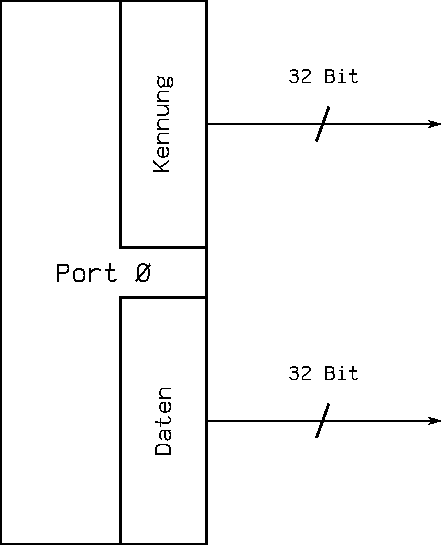
\includegraphics{./img/UMach-IOPort.pdf}
 \caption{I/O Ausgabeport}
 \label{fig:IOPort}
\end{figure}

Ein Ausgabeport besteht aus zwei Teilen, bzw. zwei Ausgängen, die jeweils 32
Bit-Signale an das angeschlossene Gerät weitergeben (siehe auch die Abbildung
\ref{fig:IOPort}):

\begin{enumerate}
 \item Kennung, die das Verwendungszweck der Daten gekennzeichnet.
 \item Daten, die den eigentlichen ausgegebenen Inhalt darstellen.
\end{enumerate}

Die Interpretation und Verwendung der Kennung und der Daten liegt in der
Verantwortlichkeit des Programmierers, der sie verwendet, bzw. des Gerätes, das
sie empfängt. Es werden seitens dieser Spezifikation keine Einschränkungen oder
Richtlinien bzgl. dieser Verwendung gegeben. Insbesondere, könnte ein Gerät die
Kennung ignorieren.
